\subsection{Testing redshift dependence of luminosity correlations}
\begin{table}[H]
\centering
\begin{tabular}{|c|c|c|c|c|c|c|c|c|}
\hline
Correlation & sample & N & a & $a_{err}$ & b & $b_{err}$ & $\sigma$ & $\sigma_{int}$\\
\hline
\multirow{3}{*}{$T_{lag}-L$} & low-z & 37 & 52.1 & 0.1 & -0.77 & 0.15 & 0.49 & 0.08\\
\cline{2-9}
 & high-z & 32 & 52.37 & 0.07 & -0.6 & 0.12 & 0.29 & 0.07\\
\cline{2-9}
 & All-z & 69 & 52.22 & 0.06 & -0.7 & 0.1 & 0.42 & 0.05\\
\hline
\multirow{3}{*}{$V-L$} & low-z & 47 & 52.12 & 0.25 & 0.65 & 0.36 & 0.91 & 0.13\\
\cline{2-9}
 & high-z & 57 & 52.63 & 0.18 & 0.25 & 0.17 & 0.63 & 0.07\\
\cline{2-9}
 & All-z & 104 & 52.34 & 0.13 & 0.46 & 0.14 & 0.75 & 0.07\\
\hline
\multirow{3}{*}{$E_{peak}-L$} & low-z & 50 & 51.89 & 0.09 & 1.43 & 0.18 & 0.59 & 0.07\\
\cline{2-9}
 & high-z & 66 & 52.23 & 0.05 & 1.09 & 0.14 & 0.34 & 0.05\\
\cline{2-9}
 & All-z & 116 & 52.05 & 0.05 & 1.35 & 0.12 & 0.5 & 0.04\\
\hline
\multirow{3}{*}{$E_{peak}-E_{\gamma}$} & low-z & 12 & 50.66 & 0.09 & 1.47 & 0.2 & 0.25 & 0.09\\
\cline{2-9}
 & high-z & 12 & 50.53 & 0.13 & 1.37 & 0.43 & 0.39 & 0.16\\
\cline{2-9}
 & All-z & 24 & 50.61 & 0.06 & 1.45 & 0.16 & 0.25 & 0.07\\
\hline
\multirow{3}{*}{$T_{RT}-L$} & low-z & 39 & 52.68 & 0.13 & -1.3 & 0.19 & 0.48 & 0.07\\
\cline{2-9}
 & high-z & 40 & 52.61 & 0.09 & -0.74 & 0.17 & 0.39 & 0.06\\
\cline{2-9}
 & All-z & 79 & 52.62 & 0.07 & -1.08 & 0.12 & 0.44 & 0.04\\
\hline
\multirow{3}{*}{$E_{peak}-E_{iso}$} & low-z & 40 & 52.57 & 0.1 & 1.55 & 0.2 & 0.6 & 0.08\\
\cline{2-9}
 & high-z & 61 & 52.74 & 0.06 & 1.2 & 0.15 & 0.4 & 0.04\\
\cline{2-9}
 & All-z & 101 & 52.65 & 0.05 & 1.42 & 0.12 & 0.49 & 0.04\\
\hline
\end{tabular}
\caption{Best fitting parameters for luminsoity correlations. N is the number of GRB samples.}
\label{table_pantheon_lstm}
\end{table}


\begin{figure}[H]
	\centering
	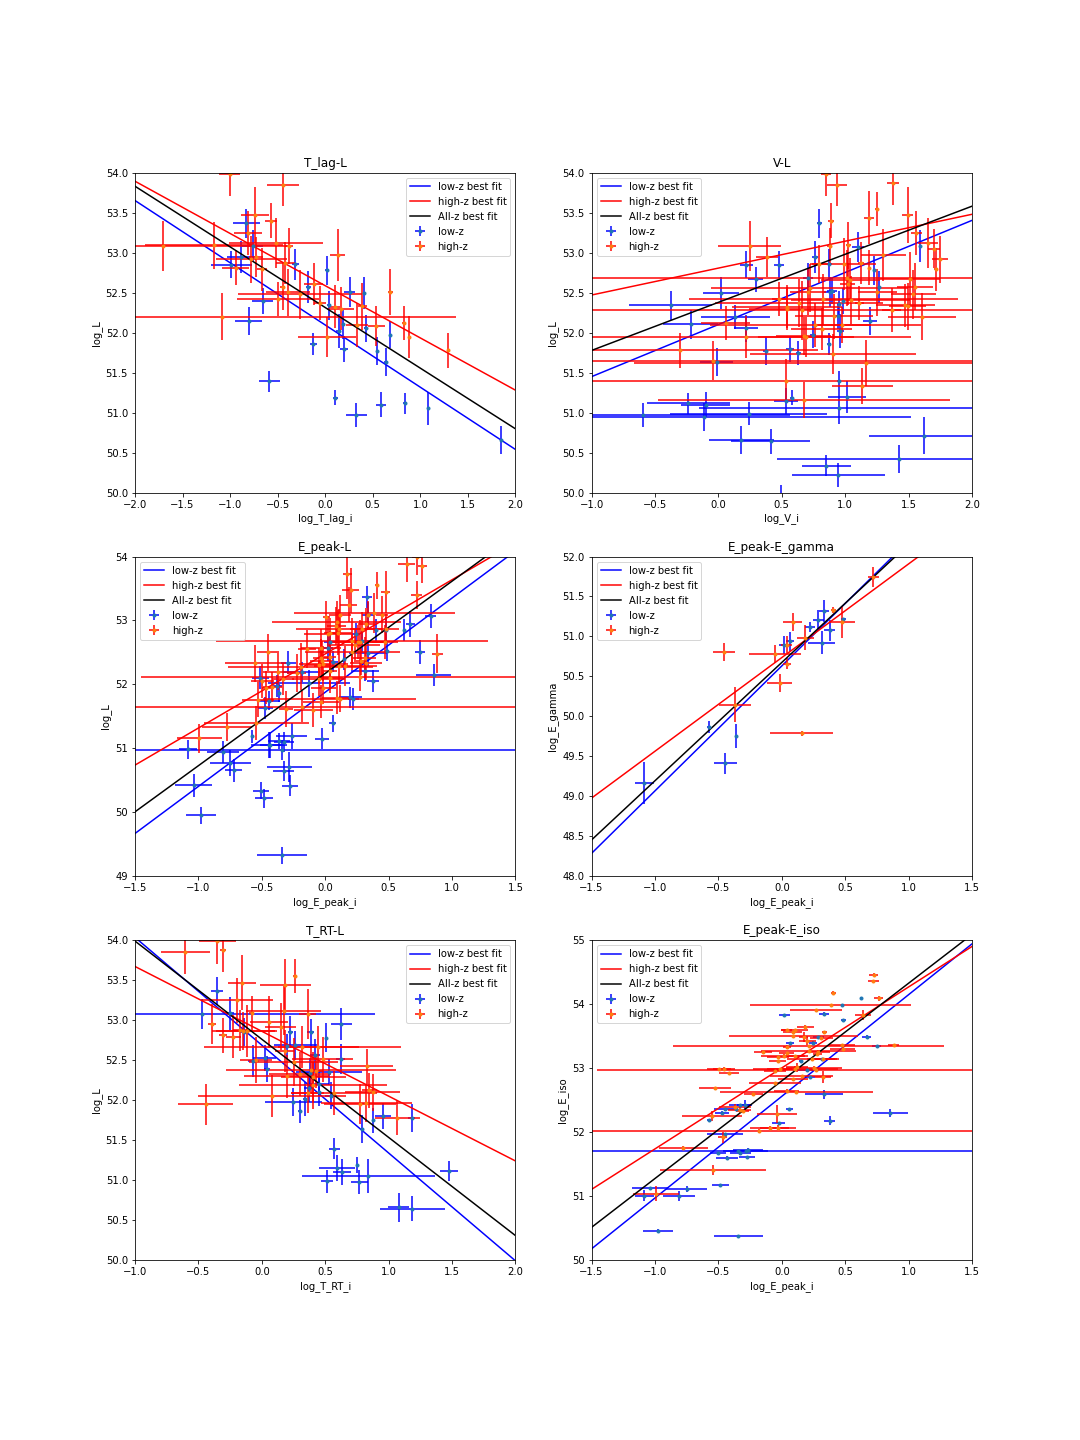
\includegraphics[width=\textwidth]{pantheon/lstm/15_correlatin.png}
	\caption{Luminsosity correlations best fit}
	\label{fig:correlation_lstm}
\end{figure}
